\section{Графы}

\subsection{Комбинаторное и топологическое описания графа}
\begin{definition}[Комбинаторное описание графа]
    $V$ — множество вершин (конечное), $E$ — множество рёбер, отношение инцидентности — любому ребру соответствует начало и конец, принадлежащие множеству вершин $V$.
\end{definition}

\begin{figure}[h]
    \centering
    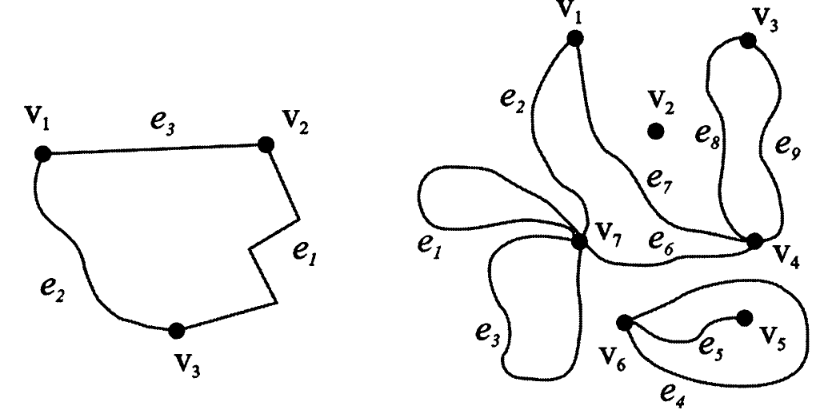
\includegraphics[scale=0.7]{images/c3.1.2.png}
    \caption{Примеры графов}
    \label{fig:c3.1}
\end{figure}

Рассмотрим рис.\ref{fig:c3.1} (граф справа):
\begin{enumerate}
    \item Вершина $v_1$ инцидентна $e_2, e_7$;
    \item Ребро $e_1$ инцидентно только $v_7$;
    \item Вершина $v_1$ смежна только с $v_4, v_7$;
    \item Ребро $e_2$ смежно только с $e_1, e_3, e_6, e_7$;
    \item Имеется ровно 3 петли: $e_1, e_3, e_4$;
    \item Кратными являются петли $e_1, e_3$ и рёбра $e_8, e_9$ (кратность равна двум);
    \item Граф справа — не простой, граф слева — простой.
\end{enumerate}

\begin{definition}
    Два графа называются \textit{изоморфными}, если существует биекция между их множествами вершин и рёбер, уважающая отношение инцидентности.
\end{definition}

$v_1, v_2 \in V_1, \ e_1 \in E_1, \ f(v_1), f(v_2) \in V_2$ если вершины $v_1$ и $v_2$ были соединены ребром $e_1$, то их образы $f(v_1)$ и $f(v_2)$ соединены ребром $f(e_1)$.

\begin{figure}[h]
    \centering
    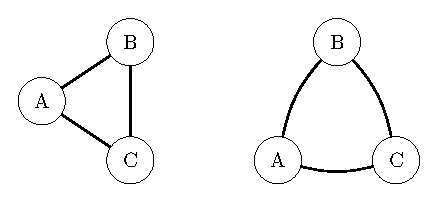
\includegraphics{images/c3.2.pdf}
    \caption{Изоморфные графы.}
    \label{fig:c3.2}
\end{figure}

\begin{definition}[Топологическое описание графа]
    Пусть дано множество (конечное) точек $V$, (конечное) множество отрезков $E$ и отображение $\partial$: (множество концов отрезков) $\to$ $V$. \textit{Графом $\Gamma(V, E, \partial)$}, определённым этими данными, назовём топологическое пространство, состоящее из множества точек $V$, называемых вершинами графа, множества внутренних точек отрезков $E$, называемых внутренними точками рёбер графа, на котором задана фактор-топология со следующим отношением эквивалентности: вершина $v$ лежит в том же классе эквивалентности, что и концы рёбер, которые в неё переходят.
\end{definition}

В теории графов принята следующая терминология:
\begin{enumerate}
    \item если $v \in \partial(e)$, то говорят, что вершина $v$ и ребро $e$ \textit{инцидентны};
    \item если $\partial(e) = \left\{v,w\right\}$, то говорят, что вершины $v$ и $w$ \textit{смежны}, или же, что они соединены ребром $e$;
    \item рёбра $e, e'$ называются \textit{смежными}, если $\partial(e) \cap \partial(e') \neq \emptyset$;
    \item ребро, инцидентное ровно одной вершине, называется \textit{петлёй};
    \item если некоторой паре вершин инцидентно несколько рёбер, то все эти рёбра называются \textit{кратными};
    \item если некоторой вершине инцидентно несколько петель, то все эти петли также называются \textit{кратными};
    \item вершина, которая инцидентна ровно одному ребру, называется \textit{висячей}.
\end{enumerate}


$v \in V, \ \partial^{-1}(v): A \sim B \Longleftrightarrow A, B \in \partial^{-1}(v), \ A \sim B \sim v$.

\begin{definition}
    Графы называются \textit{гомеоморфными}, если они гомеоморфны как топологические пространства.
\end{definition}

\begin{figure}[h]
    \centering
    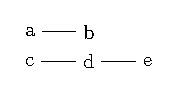
\includegraphics[scale=2]{images/c3.3.pdf}
    \caption{Гомеоморфные, но не изоморфные графы.}
    \label{fig:c3.3}
\end{figure}

\begin{definition}
    Непрерывное отображение графа $\Gamma$ в топологическое пространство $X$ называется \textit{вложением}, если при этом отображение $\Gamma$ и его образ гомеоморфны (никакие две различные точки не переходят в одну).
\end{definition}

\begin{figure}[h]
    \centering
    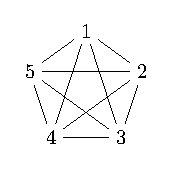
\includegraphics[scale=2]{images/c3.4.1.pdf}
    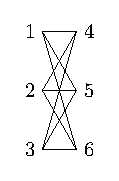
\includegraphics[scale=2]{images/c3.4.2.pdf}
    \caption{$K_5$ и $K_{3,3}$ не являются планарными.}
    \label{fig:c3.4.1,2}
\end{figure}

\begin{definition} % вне лекций
    Граф без петель и кратных рёбер называется \textit{простым}.
\end{definition}

\begin{definition}
    Граф, для которого существует его вложение в плоскость, называется \textit{планарным}.
\end{definition}

\begin{definition}
    Планарный граф вместе с вложением в плоскость называется \textit{плоским}.
\end{definition}

\begin{definition} % вне лекций
    $K_n$ — полный граф на $n$ вершинах, то есть граф, каждые две вершины которого соединены ребром.

    $K_{m,n}$ — двудольный граф, то есть граф, все вершины которого можно разбить на две группы так, что каждое ребро графа соединяет вершину из первой группы с вершиной из второй группы, при этом вершины из одной группы не имеют общих рёбер.
\end{definition}

\begin{figure}[h]
    \centering
    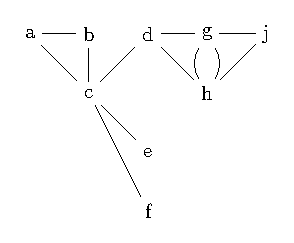
\includegraphics[scale=2]{images/c3.5.pdf}
    \caption{Имеется пять областей, на которые разбивается плоскость.}
    \label{fig:c3.5}
\end{figure}

\begin{statement}
    Любой граф можно вложить в пространство $\R^3$.
\end{statement} 
\begin{proof}
    Пусть граф $G$ без петель и кратных рёбер. Будем изображать рёбра графа отрезками. Из элементарной геометрии известно, что можно взять 4 точки так, что они не будут лежать на одной плоскости. Приняв такие точки за концы рёбер, получим, что все рёбра, у которых нет общих вершин, не пересекаются.
\end{proof} 


\subsection{Теорема о вложении планарного графа в плоскость}

\begin{theorem}
    Для связного плоского графа $B - P + \Gamma = 2$, где $\Gamma$ — количество областей, на которые граф разбивает плоскость.
\end{theorem}

\begin{theorem}[$\bigstar$]
    Для любого планарного графа существует его вложение в плоскость такое, что образ любого ребра является ломаной с конечным числом звеньев.
\end{theorem}

Свойства непрерывных кривых:

\begin{lemma}
    Образ $\gamma: [a,b] \to \R^2$ непрерывной кривой — замкнутое подмножество плоскости.
\end{lemma}
\begin{proof}
    $\left[a,b\right]$ — компакт $\Longrightarrow$ образ его — компакт.
    
    $\R^2$ — хаусдорфово $\Longrightarrow$ компакт замкнут в хаусдорфовом пространстве.

    \noindent \textit{Адаптированное доказательство из \cite{oshemkov}:} Возьмём точку $P$, которая не принадлежит образу кривой $\gamma$. Докажем, что существует такая окрестность $U$ этой точки $P$, что $U$ не пересекается с образом $\gamma$.

    Рассмотрим вспомогательную функцию $f$ на $[a,b]$, которая будет обозначать расстояние от точки $P$ до образа кривой. $f$ непрерывна $\Longrightarrow$ достигает минимума $c > 0$ (т.к. $P$ не лежит в $\gamma$). Рассмотрим тогда круг радиуса $c / 2$ с центром в $P$. Получим окрестность $U_{P, c/2}$, которая не пересекается с образом $\gamma$.
\end{proof}

%Сюда рисунок №6

\begin{lemma}[о первой точке]
    $\Omega$ — замкнутое подмножество $\R^2$, $\gamma(t)$ — непрерывная кривая, $\gamma: [0,1] \to \R^2, \ \gamma(0) = A \notin \Omega, \ \gamma(1) = B \in \Omega \Longrightarrow \exists t_0 \in  [0,1]: \ \gamma(t_0) \in \Omega, \ \forall t < t_0 \ \gamma(t) \notin \Omega$.
\end{lemma}
\begin{proof}
    Рассмотрим $T: \left\{
        \tau \in [0,1]: \ \forall t \in [0, \tau): \ \gamma(t) \notin \Omega
    \right\}$ — не пусто (так как $0 \in T$) и ограничено.

    Так как множество $T$ не пусто и ограничено, то можно сказать, что существует $\sup{T} = c$, более того, $c \neq 1$, т.к. $\gamma(1) = B \in \Omega$ по условию.

    Если $\gamma(c) = C \notin \Omega$, то существует окрестность $U$ точки $C$ такая, что $U \cap \Omega = \emptyset$ (воспользовались замкнутостью множества $\Omega$).

    Так как $\gamma$ — непрерывная кривая, то существует окрестность $V = (c - \epsilon, c + \epsilon)$ такая, что $\gamma(V) \in U$, то есть $\forall t \in (c - \epsilon, c + \epsilon): \gamma(t) \notin \Omega \Longrightarrow c \neq \sup{T}$ — противоречие, значит, $C \in \Omega$.
    
    В качестве $t_0$ возьмём $c$.

    % (В исходнике есть наброски прямо с лекции)
    %$U$ — окрестность точки $A$: $U \cap \Omega = \emptyset \ \exists \tau_0: \ \gamma(t) \in U \Longrightarrow t \in [0, \tau_0) \ \gamma(t) \notin \Omega, 0 \leq t < \tau_0$.
    %$\sup{\tau} = t_0$. Пусть $\gamma(t_0) \notin \Omega$, тогда существует $V$ окрестность $\gamma(t_0) \notin \Omega \Longrightarrow \exists \delta \ \forall t \in (t_0 - \delta, t_0 + \delta), \ \gamma(t) \in V \Longrightarrow \gamma(t) \notin \Omega, \ \gamma(t_0 + \frac{\delta}{2}) \notin \Omega \Longrightarrow t_0$ — не супремум.
\end{proof}

\begin{proof}[Доказательство $\bigstar$]
    %Адаптация лекционного доказательства, основанная на \cite{oshemkov}.
    % Пока не готово, можете посмотреть у Ошемкова \cite{oshemkov}.
    
    % Шаг 1. Удалим из графа петли.
    
    % Шаг 2. Сюда рисунок №7. Для каждой вершины рассмотрим окрестность такую, что она не пересекается с рёбрами графа, НЕ инцидентными данной вершине, и другими вершинами. Рассмотрим замкнутые окрестности вершин в два раза меньшего радиуса.

    % Шаг 3. Исправляем вложение в окрестности вершины и добавим обратно петли. Сюда рисунок №8

    % Шаг 4. Сюда рисунок №9. Рассмотрим две окрестности вершин, соединённых ребром. Хотим заменить $\gamma: [0,1] \to \R^2, \ \gamma(0) = A, \ \gamma(1) = B$ на ломаную.
    % Рассмотрим 
    % % \begin{multline}
    % %     T = \left\{
    % %     \tau \in [0,1]: \gamma(0) = A \ \text{и} \ \gamma(\tau) \text{могут быть соединены вложенной} \\ \text{конечнозвенной ломаной, не пересекающей другие рёбра графа}
    % % \right\}
    % % \end{multline}
    % $T$ не пусто, так как содержит ноль.

    % $T$ открыто: $\tau_0 \in T, \ \exists \epsilon: \ \forall \tau \in B_{\epsilon}(\tau_0)$, $\gamma(\tau)$ можно соединить с $A$, выберем окрестность $U$ точки $C = \gamma(\tau_0)$

    Пусть заданный граф не имеет петель. Если они есть, то удалим их, а потом вернём.

    Для каждой вершины рассмотрим окрестность такую, что она не пересекается с рёбрами графа, НЕ инцидентными данной вершине $v$, и другими вершинами. Рассмотрим замкнутые окрестности вершин в два раза меньшего радиуса $D_v$.

    Так как ребро, выходящее из вершины $v$ — непрерывная кривая, то по лемме о первой точке на этой кривой будет первая точка, которая принадлежит замкнутому кругу $D_v$. Изменим вложение для этого ребра на отрезке между $v$ и первой точкой на радиус (см.рис.\ref{fig:c3.6}). Сделаем так для всех рёбер. На этом моменте можно вернуть петли, изображённые ломаными.

    \begin{figure}[h]
        \centering
        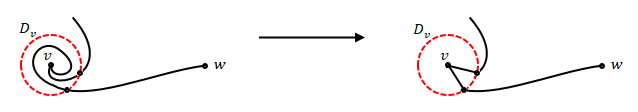
\includegraphics[scale=0.7]{images/c3.6.png}
        \caption{Изменение вложения в окрестности вершины}
        \label{fig:c3.6}
    \end{figure}

    Теперь надо поменять вложение на остальных частях рёбер (та, которая лежит между нашими замкнутыми окружностями). Если мы для каждого отдельного ребра докажем, что можем поменять вложение, которое было, на ломаную, не трогая остальных рёбер, то докажем теорему (см.рис.\ref{fig:c3.7}).

    \begin{figure}[h]
        \centering
        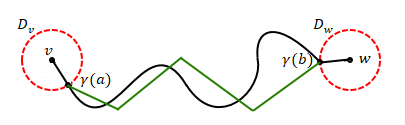
\includegraphics[scale=0.7]{images/c3.7.png}
        \caption{Изменение вложения на остальных частях рёбер}
        \label{fig:c3.7}
    \end{figure}

    Рассмотрим ребро, соединяющее вершины $v, w$. Средняя часть — непрерывная кривая $\gamma: [a,b] \to \R^2$ \footnote{Здесь и далее в лекциях дан отрезок [0,1], но, очевидно, это ни на что не повлияет, просто мне пока что лень рисовать свои рисунки, поэтому я их просто позаимствовал в \cite{oshemkov}}. Рассмотрим множество: $T = \{t \in [a,b]\}$, где $t$ такие, что $\gamma(a)$ можно соединить ломаной с $\gamma(t)$ так, что эта ломаная не имеет самопересечений и не пересекает другие рёбра.
    $T$ не пусто хотя бы потому, что $t = a$ условие выполняется.
    Докажем, что и $b$ принадлежит $T$.
    Идея дальнейшего доказательства состоит в том, чтобы отступать от левого конца отрезка, чтобы потом добраться до правого конца.

    \begin{figure}[h]
        \centering
        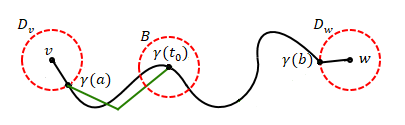
\includegraphics[scale=0.7]{images/c3.8.png}
        \caption{Изменение вложения на остальных частях рёбер}
        \label{fig:c3.8}
    \end{figure}

    Сначала докажем, что если $t_0 \in T$, то и $(t_0 - \epsilon, t_0 + \epsilon) \subset T$ для некоторого $\epsilon > 0$ (иными словами, докажем, что множество $T$ — открытое подмножество $[a,b]$).

    Рассмотрим на кривой $\gamma$ точку $\gamma(t_0)$ и замкнутый круг $B$ с центром в этой точке, который не пересекает другие рёбра и круги $D_v$ (это возможно, так как образы других рёбер — замкнутые подмножества плоскости).

    По предположению $t_0 \in T$, тогда существует ломаная, которая идёт от $a$ до $t_0$.
    Тогда мы можем соединить $\gamma(a)$ с любой точкой круга $B$ хорошей ломаной (не имеющей самопересечений и пересечений с другими рёбрами) по ломаной из $\gamma(a)$ в $\gamma(t_0)$ до первой её точки в круге $B$ и далее по отрезку.

    С другой стороны (по определению непрерывности кривой), для круга $B$ существует интервал $(t_0 - \epsilon, t_0 + \epsilon)$ такой, что его образ содержится в этом круге — стало быть, доказали, что если $t_0 \in T$, то $(t_0 - \epsilon, t_0 + \epsilon) \subset T$, то есть, $T$ — открытое подмножество на $[a,b]$.

    Далее докажем (аналогично), что если $t_0 \notin T$, то для некоторого $\epsilon > 0$ выполнено $(t_0 - \epsilon, t_0 + \epsilon) \cap T = \emptyset$, то есть, что дополнение $[a,b] \setminus T$ тоже открыто в $[a,b]$.
    Предположим, что $\gamma(t_0)$ не принадлежит множеству $T$.
    Рассмотрим круг с центром в точке $\gamma(t_0)$, который не пересекается с остальными рёбрами, и рассмотрим интервал $(t_0 - \epsilon, t_0 + \epsilon)$, который при отображении $\gamma$ целиком попадает в этот круг.

    Мы не можем соединить $\gamma(a)$ хорошей ломаной с точками из этого интервала, если не можем соединить $\gamma(a)$ с точкой $\gamma(t_0)$ — действительно, иначе дойдём до первой точки круга с центром в точке $\gamma(t_0)$, и далее дойдём до точки $\gamma(t_0)$.
    Таким образом, если $t_0 \notin T$, то и $t \notin T$, где $t \in (t_0 - \epsilon, t_0 + \epsilon)$.

    Тем самым мы доказали, что множества $T$ и $[a,b] \setminus T$ открыты в $[a,b]$.
    Теперь докажем, что если $T \subset [a,b]$ и $([a,b] \setminus T) \subset [a,b]$ — открытые множества в $[a,b]$, то одно из них пусто.

    Действительно, рассмотрим
    \[\sup(t \in [a,b]: \ [a,t] \in T) = c.\]
    Иными словами, рассмотрим отрезок $[a,b]$ и, поскольку мы знаем, что $a \in T$, будем идти по отрезку, пока мы находимся в множестве $T$.

    Если $c \in T$ и $c \neq b$, то как мы доказали, $(c - \epsilon, c + \epsilon) \subset T$ для $\epsilon > 0$, а значит, $c$ не является верхней гранью для этого множества. Значит, если $c < b$, то $c$ не может принадлежать $T$.

    Аналогично, если $c \notin T$, то есть $c \in [a,b] \setminus T$, то $(c - \epsilon, c + \epsilon) \subset [a,b] \setminus T$, то есть $c$ — не точная верхняя грань, поскольку, например, $c - \epsilon$ — верхняя грань.
    Поэтому $c = b$, так как $[a,b] \setminus T$ открыто и не может состоять только из одной точки — правого конца отрезка.

\end{proof}

% конец третьей лекции